\chapter{Técnicas de visión computerizada}
Aquí se detallan todas las técnicas aplicadas o descartadas a lo largo
de la investigación. Incluye ejemplos de las tomografías para poder
relacionar la técnica con el resultado visual.\\
Toda la información presente en este capítulo ha sido redactada acorde
a las siguientes fuentes:
% TODO: Falta añadir bibliografías de Learn OpenCV, el tutorial de
% Python y la API

\section{Conocimientos previos necesarios}

\subsection{Histogramas}
Un histograma es un gráfico con la distribución de color o
intensidades de la imagen, por simplificación, suponemos siempre una
imagen en escala de grises. Es tan importante su estudio dentro de la
visión computerizada que se podría definir informalmente como el
gráfico que contiene la naturaleza de la imagen.
\begin{description}
\item[Columnas:] representan intensidades. Cada columna tiene una
  altura que corresponde proporcionalmente a la cantidad de píxeles
  con dicho valor.
\item[Dimensiones:] parámetros o número de datos a mostrar en el
  histograma. En el caso de una escala de grises sólo hay una
  dimensión, la intensidad, que puede ser 1 si el píxel tiene dicha
  intensidad o 0 en caso contrario.
\item[Rango:] es el número de columnas. En escala de grises el rango
  es de 256 columnas desde 0 hasta 255.
\end{description}

\subsubsection{Cálculo}
Para realizar el cálculo de un histograma y por simplificación se usa
una biblioteca. Tanto \emph{Numpy} como \emph{OpenCV} son capaces de
realizar los cálculos necesarios pero por eficiencia se usa
\emph{OpenCV}.

\subsubsection{Dibujado}
El resultado de un histograma es una matriz de \emph{Numpy} por lo que,
para poder dibujarla, tiene que usarse \emph{Matplotlib} o transformar
la matriz en una imagen de \emph{OpenCV}.

\subsubsection{Ecualización}
La ecualización de un histograma consiste en distribuir los píxeles
por todo el rango. Esta acción aumenta el contraste en aquellas
imágenes que tienen la mayoría confinados en una zona pequeña del
rango.

\subsection{Convolución de matrices}
La \emph{convolución} de una matriz sobre una imagen, que al fin y al
cabo es otra matriz, es la principal base de la mayoría de las
técnicas aquí descritas. \\
Un \emph{kernel} es una matriz fija de coeficientes numéricos y 
dimensión \textbf{impar} que se usa en todas las técnicas de este capítulo 
para tener un elemento como el elemento central. \\
Para calcular la convolución de un píxel concreto se sitúa éste en el
centro del \emph{kernel} y se calcula su valor con respecto a los
píxeles de alrededor, multiplicando su valor por el valor del
\emph{kernel} para esa posición. Finalmente, cada multiplicación se
suma y se guarda el resultado total en la posición central. Este
proceso se repite con cada píxel. \\
La ecuación que representa el proceso anterior, definiendo la imagen
como $I(x, y)$, el \emph{kernel} como $K(i, j)$ (donde
$0 < i < M_j - 1$ y $0 < j < M_j - 1$) y el centro de la matriz de
convolución es $(c_i, c_j)$ definimos la imagen resultante como
\begin{equation*}
  R(x, y) = \sum_{i=0}^{M_i-1} \sum_{j=0}^{M_j-1}  I(x + i - c_i, y + j - c_j)K(i,j)
\end{equation*}
En el caso de \emph{OpenCV}, tanto la imagen original \emph{I} como la
imagen resultante \emph{R} son del mismo tamaño. Esto se debe a que
\emph{OpenCV} duplica el borde de manera virtual para que el
\emph{kernel} de convolución se pueda aplicar hasta el mismo borde de
la imagen. Hay distintas maneras de duplicar el borde pero aquí sólo
se muestra la más simple y sobre el eje de abscisas:
\begin{center}
  $imagen(-dx, y) = imagen(0, y)$
  \\
  $imagen(w + dx) = imagen(w - 1, y)$
\end{center}


\section{Operaciones básicas}
\subsection{Acceso a píxeles}
El acceso a los píxeles de una imagen se realiza a través de
\emph{Numpy} como una matriz de dimensiones [\emph{y}, \emph{x}],
siendo \emph{y} la altura y \emph{x} el ancho.
\begin{minted}{Python}
  pixel = imagen[y, x]
\end{minted}

\subsection{Propiedades}
Las dos propiedades más utilizadas de las imágenes son su altura y
anchura.  Se pueden obtener con la función \emph{shape}.
\begin{minted}{Python}
  y, x = imagen.shape
\end{minted}

\subsection{Región de interés}
La región de interés (ROI) de una imagen es la zona que estamos
interesados en procesar. Se expresa mediante los vértices opuestos de
un rectángulo o cuadrado definidos como los píxeles [$y_1$, $x_1$] y
[$y_2$,$x_2$] de la imagen
\begin{minted}{Python}
  roi = imagen[y1:y2, x1:x2]
\end{minted}

\section{Operaciones aritméticas}
\subsection{Superposición}
La superposición de dos imágenes (del mismo tipo, profundidad o una
que sea un valor escalar) es la suma matricial de sus píxeles,
asignando a cada imagen un peso diferente para dar la sensación de
superposición y transparencia. La función sería:
\begin{equation*}
  g(n) = (1 - \alpha)f_0(n) + \alpha f_1(n)
\end{equation*}
Donde \emph{n} representa un punto de la imagen, \emph{$\alpha$} es
una constante entre 0 y 1, y \emph{$f_0$} y \emph{$f_1$} las imágenes.
Expresado en forma de coordenadas:
\begin{equation*}
  g(x, y) = (1 - \alpha)f_0(x, y) + \alpha f_1(x, y)
\end{equation*}
Donde \emph{x} e \emph{y} representan las coordenadas (horizontal y
vertical respectivamente).


\section{Cambio de espacio de color}
Un espacio de color es un modelo matemático abstracto que describe la
forma en la que los colores pueden representarse como tuplas de
números. RGB, HSV o escala de grises son ejemplos de espacios de color. \\
El espacio de color de una imagen se puede cambiar con la función
\emph{cvtColor}. Esta función permite las siguientes conversiones en
las dos direcciones:
\begin{itemize}
\item \textbf{RGB} --- \textbf{escala de grises}.
\item \textbf{RGB} --- \textbf{CIE XYZ}.
\item \textbf{RGB} --- \textbf{YCrCb JPEG} (o YCC).
\item \textbf{RGB} --- \textbf{HSV}.
\item \textbf{RGB} --- \textbf{HLS}.
\item \textbf{RGB} --- \textbf{Bayer}.
\end{itemize}
Estas transformaciones permiten la detección rápida y sencilla de
características de interés. \\
Para este proyecto se han usado las que implican RGB y escala de
grises.

\section{Operaciones de \emph{threshold}}
Las operaciones de \emph{threshold} convierten los píxeles de una
imagen (en escala de grises [0 --- 255]) superiores a un valor,
conocido como valor de umbral, a blanco [255] o a negro [0], según el
\emph{threshold} aplicado.
\subsection{Simples}
\subsubsection{cv2.THRESH\_BINARY}
Todos los píxeles con un valor mayor que el valor de umbral se
transforman, asignándoles el valor máximo. Los que no lo superen,
adquieren el valor mínimo.  La expresión es
\begin{equation*}
  destino(x, y) =
  \begin{cases}
    255 & \text{si } entrada(x, y) > umbral \\
    0 & \text{cualquier otro caso}
  \end{cases}
\end{equation*}
Ejemplo para un valor de umbral de 127 (Arriba original y abajo el resultado
obtenido tras aplicar el filtro):

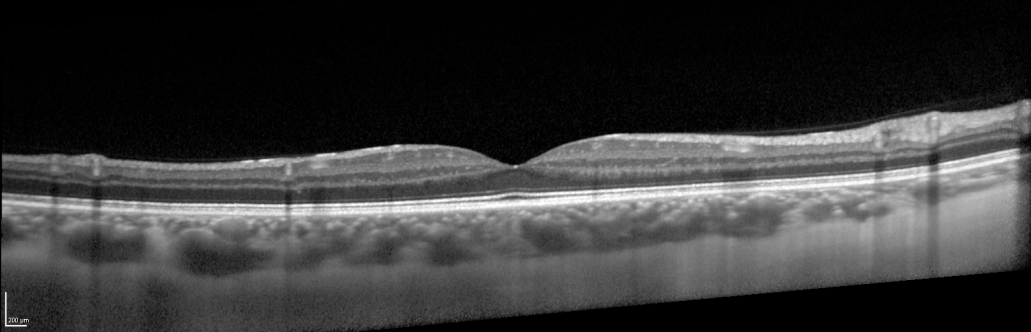
\includegraphics[scale=0.40]{imagenes/EjemploTecnicasThresholdOriginal.png}\\
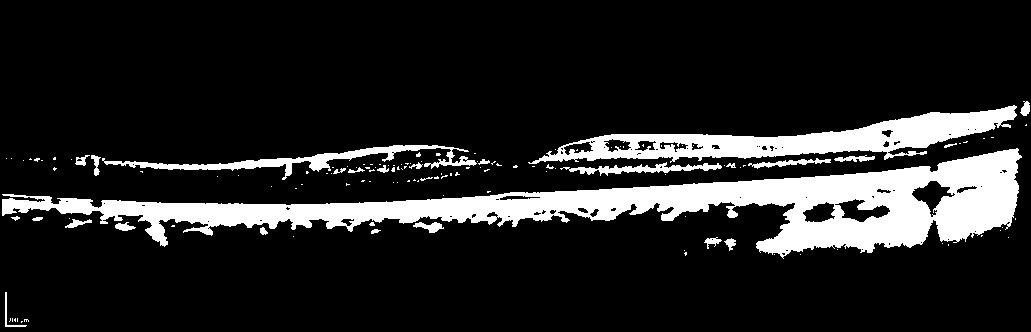
\includegraphics[scale=0.40]{imagenes/EjemploTecnicasThresholdBinary_127.png}

\subsubsection{cv2.THRESH\_BINARY\_INV}
Es la operación contraria al anterior: a los píxeles con un valor
mayor que el valor de umbral se les asigna el valor mínimo, mientras
que los demás adquieren el valor máximo. La expresión es
\begin{equation*}
  destino(x, y) =
  \begin{cases}
    0 & \text{si } entrada(x, y) > umbral \\
    255 & \text{cualquier otro caso}
  \end{cases}
\end{equation*}
Ejemplo para un valor de umbral de 127 (Arriba original y abajo el resultado
obtenido tras aplicar el filtro):

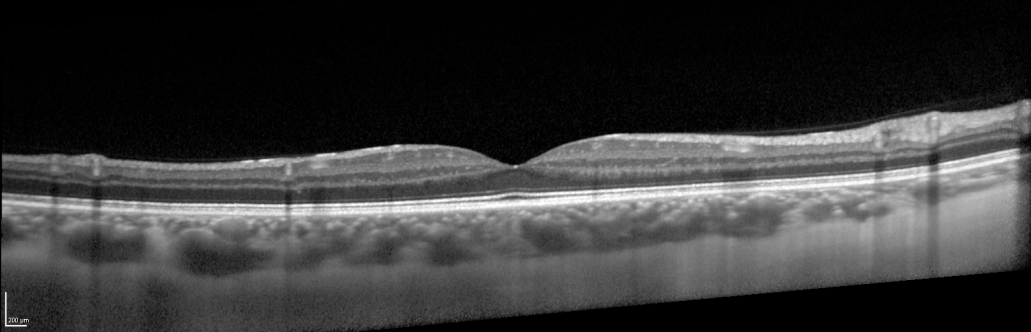
\includegraphics[scale=0.40]{imagenes/EjemploTecnicasThresholdOriginal.png}\\
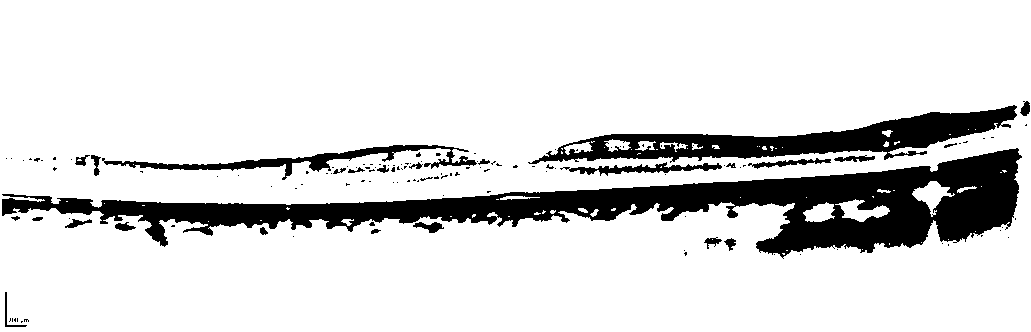
\includegraphics[scale=0.40]{imagenes/EjemploTecnicasThresholdBinaryInv_127.png}


\subsubsection{cv2.THRESH\_TRUNC}
Se trunca el valor de los píxeles de forma que todos los píxeles que
superen el valor de umbral toman dicho valor. En caso contrario se
conserva el valor original. La expresión es
\begin{equation*}
  destino(x, y) =
  \begin{cases}
    umbral & \text{si } entrada(x, y) > umbral \\
    entrada(x, y) & \text{cualquier otro caso}
  \end{cases}
\end{equation*}
Ejemplo para un valor de umbral de 127 (Arriba original y abajo el resultado
obtenido tras aplicar el filtro):

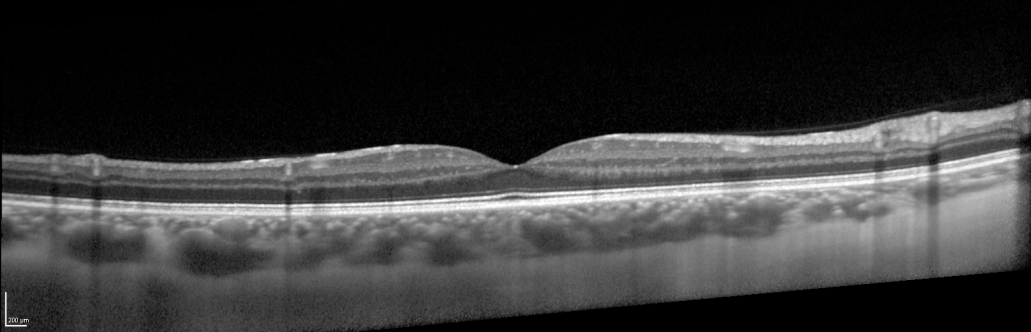
\includegraphics[scale=0.40]{imagenes/EjemploTecnicasThresholdOriginal.png}\\
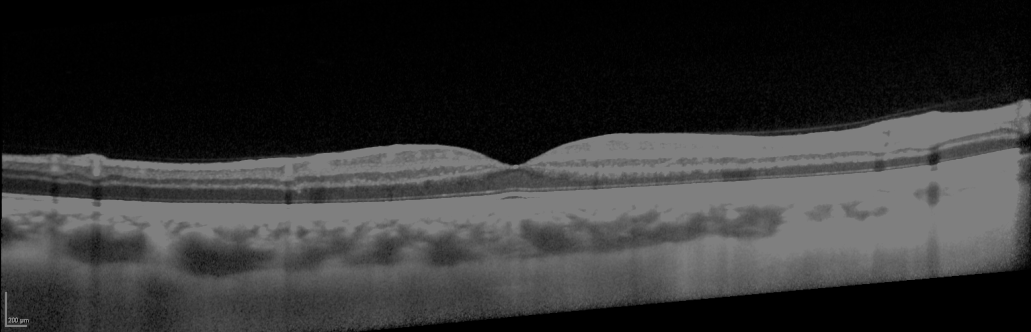
\includegraphics[scale=0.40]{imagenes/EjemploTecnicasThresholdTrunc_127.png}


\subsubsection{cv2.THRESH\_TOZERO}
Es la operación contraria a la anterior: los píxeles que superen el
valor del umbral conservan su valor original, mientras que en el caso
contrario se les aplica el valor mínimo. La expresión es
\begin{equation*}
  destino(x, y) =
  \begin{cases}
    entrada(x, y) & \text{si } entrada(x, y) > umbral \\
    0 & \text{cualquier otro caso}
  \end{cases}
\end{equation*}
Ejemplo para un valor de umbral de 127 (Arriba original y abajo el resultado
obtenido tras aplicar el filtro):

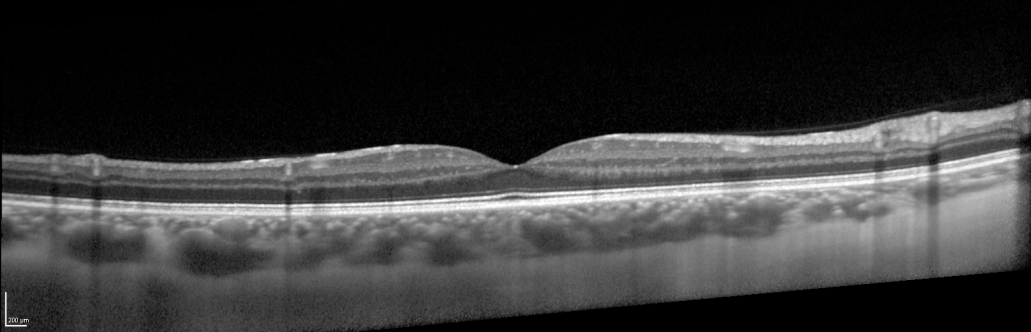
\includegraphics[scale=0.40]{imagenes/EjemploTecnicasThresholdOriginal.png}\\
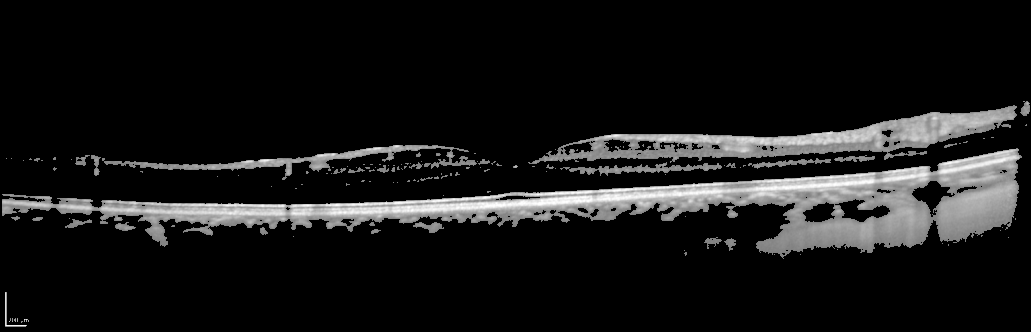
\includegraphics[scale=0.40]{imagenes/EjemploTecnicasThresholdTo0_127.png}


\subsubsection{cv2.THRESH\_TOZERO\_INV}
A los píxeles que superen el valor de umbral se les aplica el valor
mínimo, mientras que en caso contrario conservan el valor original. La
expresión es
\begin{equation*}
  destino(x, y) =
  \begin{cases}
    0  & \text{si } entrada(x, y) > umbral \\
    entrada(x, y) & \text{cualquier otro caso}
  \end{cases}
\end{equation*}
Ejemplo para un valor de umbral de 127 (Arriba original y abajo el resultado
obtenido tras aplicar el filtro):

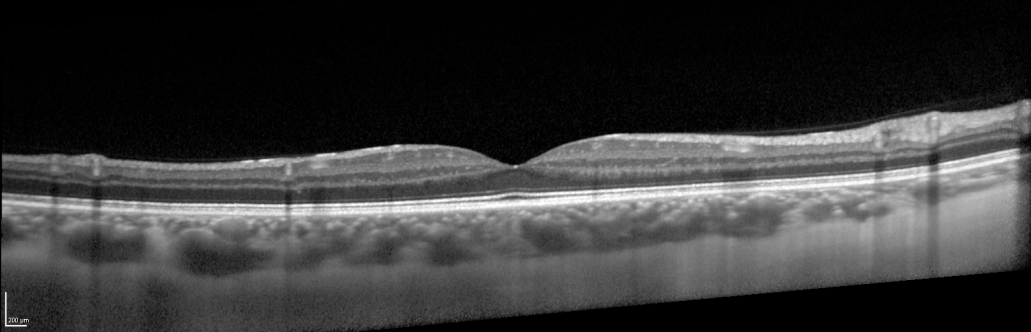
\includegraphics[scale=0.40]{imagenes/EjemploTecnicasThresholdOriginal.png}\\
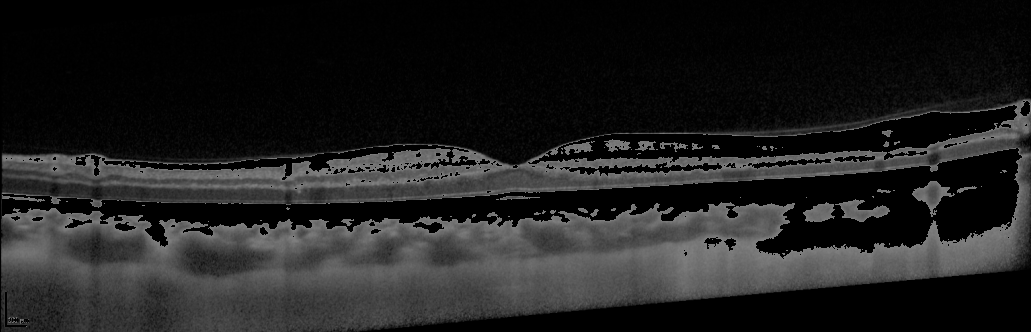
\includegraphics[scale=0.40]{imagenes/EjemploTecnicasThresholdTo0Inv_127.png}

\subsection{Adaptativos}
En imágenes uniformes aplicar valores umbral globales y fijos suele
ser una buena opción pero para imágenes no uniformes hay que adaptar
dicho valor a cada área de la imagen. Por ello, se aplican las dos
técnicas siguientes. En ambas, el área a realizar el \emph{threshold}
depende del tamaño del \emph{kernel} usado.

\subsubsection{cv2.ADAPTIVE\_THRESH\_MEAN\_C}
El valor de cada píxel se establece por la media de sus vecinos.

\subsubsection{cv2.ADAPTIVE\_THRESH\_GAUSSIAN\_C}
El valor de cada píxel se establece por el resultado de una función
Gaussiana a partir de sus vecinos.

\subsection{ Otsu}
Este \emph{threshold} calcula el valor umbral a partir del histograma
de la imagen. La precisión de esta técnica depende de que el
histograma sea lo más bimodal posible, en los que predomina dos
columnas.

\section{Transformaciones geométricas}
Las transformaciones geométricas son aquellas técnicas en las que se
aplica una matriz o \emph{kernel} de transformación a la imagen
original.
\subsection{Rotación}
Para rotar una imagen desde un ángulo $\theta$ se opera con la
siguiente matriz de transformación.
\begin{equation*}
  M =
  \begin{bmatrix}
    \cos \theta & -\sin \theta \\ \sin \theta & \cos \theta
  \end{bmatrix}
\end{equation*}
\emph{OpenCV} además, facilita una matriz de rotación escalable con
centro ajustable para el punto que se prefiera.
\begin{equation*}
  \begin{bmatrix}
    \alpha & \beta & (1 - \alpha) \cdot centro_x - \beta \cdot centro_y \\
    - \beta & \alpha & \beta \cdot centro_x + (1 - \alpha) \cdot
    centro_y
  \end{bmatrix}
\end{equation*}
donde:
\begin{center}
  $ \alpha = escala \cdot \cos \theta $
  \\
  $ \beta = escala \cdot \sin \theta $
\end{center}
Para facilitar todavía más la rotación, \emph{OpenCV} proporciona la
función
\begin{center}
  \textbf{cv2.getRotationMatrix2D}(centro, ángulo, escala) \\
  $\downarrow$ \\
  matriz de transformación
\end{center}
Posteriormente hay que aplicar la función de afinidad con la matriz de transformación anterior \\
\begin{center}
  \textbf{cv2.warpAffine}(imagen, matriz, tamaño)\\
  $\downarrow$ \\
  imagen destino
\end{center}

\section{\emph{Blur}}
\emph{Blur} o suavizado es una técnica usada con el objetivo principal
de reducir el ruido y los artefactos (contenido de alta frecuencia) de
la imagen, aunque también se usa para disminuir la resolución. Se basa
en aplicar a la imagen un \emph{kernel} de convolución.
\subsection{Basado en la media}
En el caso de un \emph{blur}, se suman todos los valores de los
píxeles contenidos en la matriz y se divide entre el número de
vecinos. El \emph{kernel} a aplicar es el siguiente
\begin{equation*}
  K = \frac{1}{n}
  \begin{bmatrix}
    1_{11} & 1_{12} & \cdots & 1_{1n} \\
    1_{21} & 1_{22} & \cdots & 1_{2n} \\
    \vdots & \vdots & \ddots & \vdots \\
    1_{n1} & 1_{n2} & \cdots & 1_{nn} \\
  \end{bmatrix}
  \text{siendo \emph{n} un número \textbf{impar}}
\end{equation*}

A modo de ejemplo, el \emph{kernel} de dimensión $3\times3$ es
\begin{equation*}
  K = \frac{1}{9}
  \begin{bmatrix}
    1 & 1 & 1 \\
    1 & 1 & 1 \\
    1 & 1 & 1 \\
  \end{bmatrix}
\end{equation*}
\subsection{Basado en una función Gaussiana}
Esta técnica es la que mejor resultados suele dar y especialmente si
se utiliza para reducir ruido generado por un \emph{kernel
  Gaussiano}. Cabe destacar que al aplicar este método puede darse
como resultado valores de píxeles que no estuvieran en la imagen
original. Este \emph{Blur} es el menos eficiente de todos pero
\emph{OpenCV} lo optimiza para las sigmas $\sigma_x$ e $\sigma_y$
predeterminadas para los \emph{kernels} de $3\times3$, $5\times5$ y
$\times7$. Debido a esto, sólo mostraremos como se
generan estas sigmas predeterminas y un ejemplo con ellas.\\
\emph{OpenCV} obliga a introducir $\sigma_x$ y en el caso de que este
sea 0, se determinan ambos sigmas a partir del tamaño del
\emph{kernel} introducido mediante las fórmulas siguientes:
\begin{equation*}
  \sigma_x = \left(\frac{n_x}{2} - 1 \right) \cdot 0,30 + 0.80, n_x = \text{anchura del \emph{kernel}}
\end{equation*}
\begin{equation*}
  \sigma_y = \left(\frac{n_y}{2} - 1 \right) \cdot 0,30 + 0.80, n_y = \text{altura del \emph{kernel}}
\end{equation*}

\subsection{Basado en la mediana}
En el caso de un \emph{median Blur} y como oposición al \emph{Blur},
,que se basa en la media, el \emph{median Blur} calcula el valor
del píxel central mediante la mediana de los píxeles colindantes. \\
Esta técnica es muy útil para reducir el ruido granulado de la imagen.

\section{Transformaciones morfológicas}
Las operaciones de transformación morfológicas se aplican sobre la
forma de la imagen. Se suelen usar para reducir el ruido, aislar o
juntar elementos. El \emph{kernel} aplicado a la imagen define el
resultado de la operación. Para enteder mejor la operación supondremos
que la imagen está \emph{binarizada} (píxeles únicamente blancos o
negros)
\subsection{\emph{Erosion}}
\subsection{\emph{Dilation}}
\subsection{\emph{Opening}}
\subsection{\emph{Closing}}
\subsection{Gradiente morfológico}

\section{Gradientes}
\subsection{Sobel}
\subsection{Scharr}
\subsection{Laplaciana}

\section{Algoritmo \emph{Canny}}

\section{Contornos}

\section{Transformada de Hough}
\subsection{Rectas}